\chapter{XSD}

Dans cette partie, nous expliquerons notre conception de la partie validation d'une document xml avec un document xsd. Voici les hypothèses simplificatrices dont nous avons tenu compte :
\begin{itemize}
    \item{les types de base seront uniquement de type string ou date}
    \item{les types complexes seront uniquement de type sequence ou choice}
\end{itemize}
De plus, nous avons choisi de traiter les points optionnels suivants suivants :
\begin{itemize}
    \item{les éléments de types mixed sont autorisés}
    \item{les attributs seront vérifiés}
\end{itemize}

\section{Conception}

    \subsection{Diagramme de classe}

    \begin{figure}[H]
        \centering
        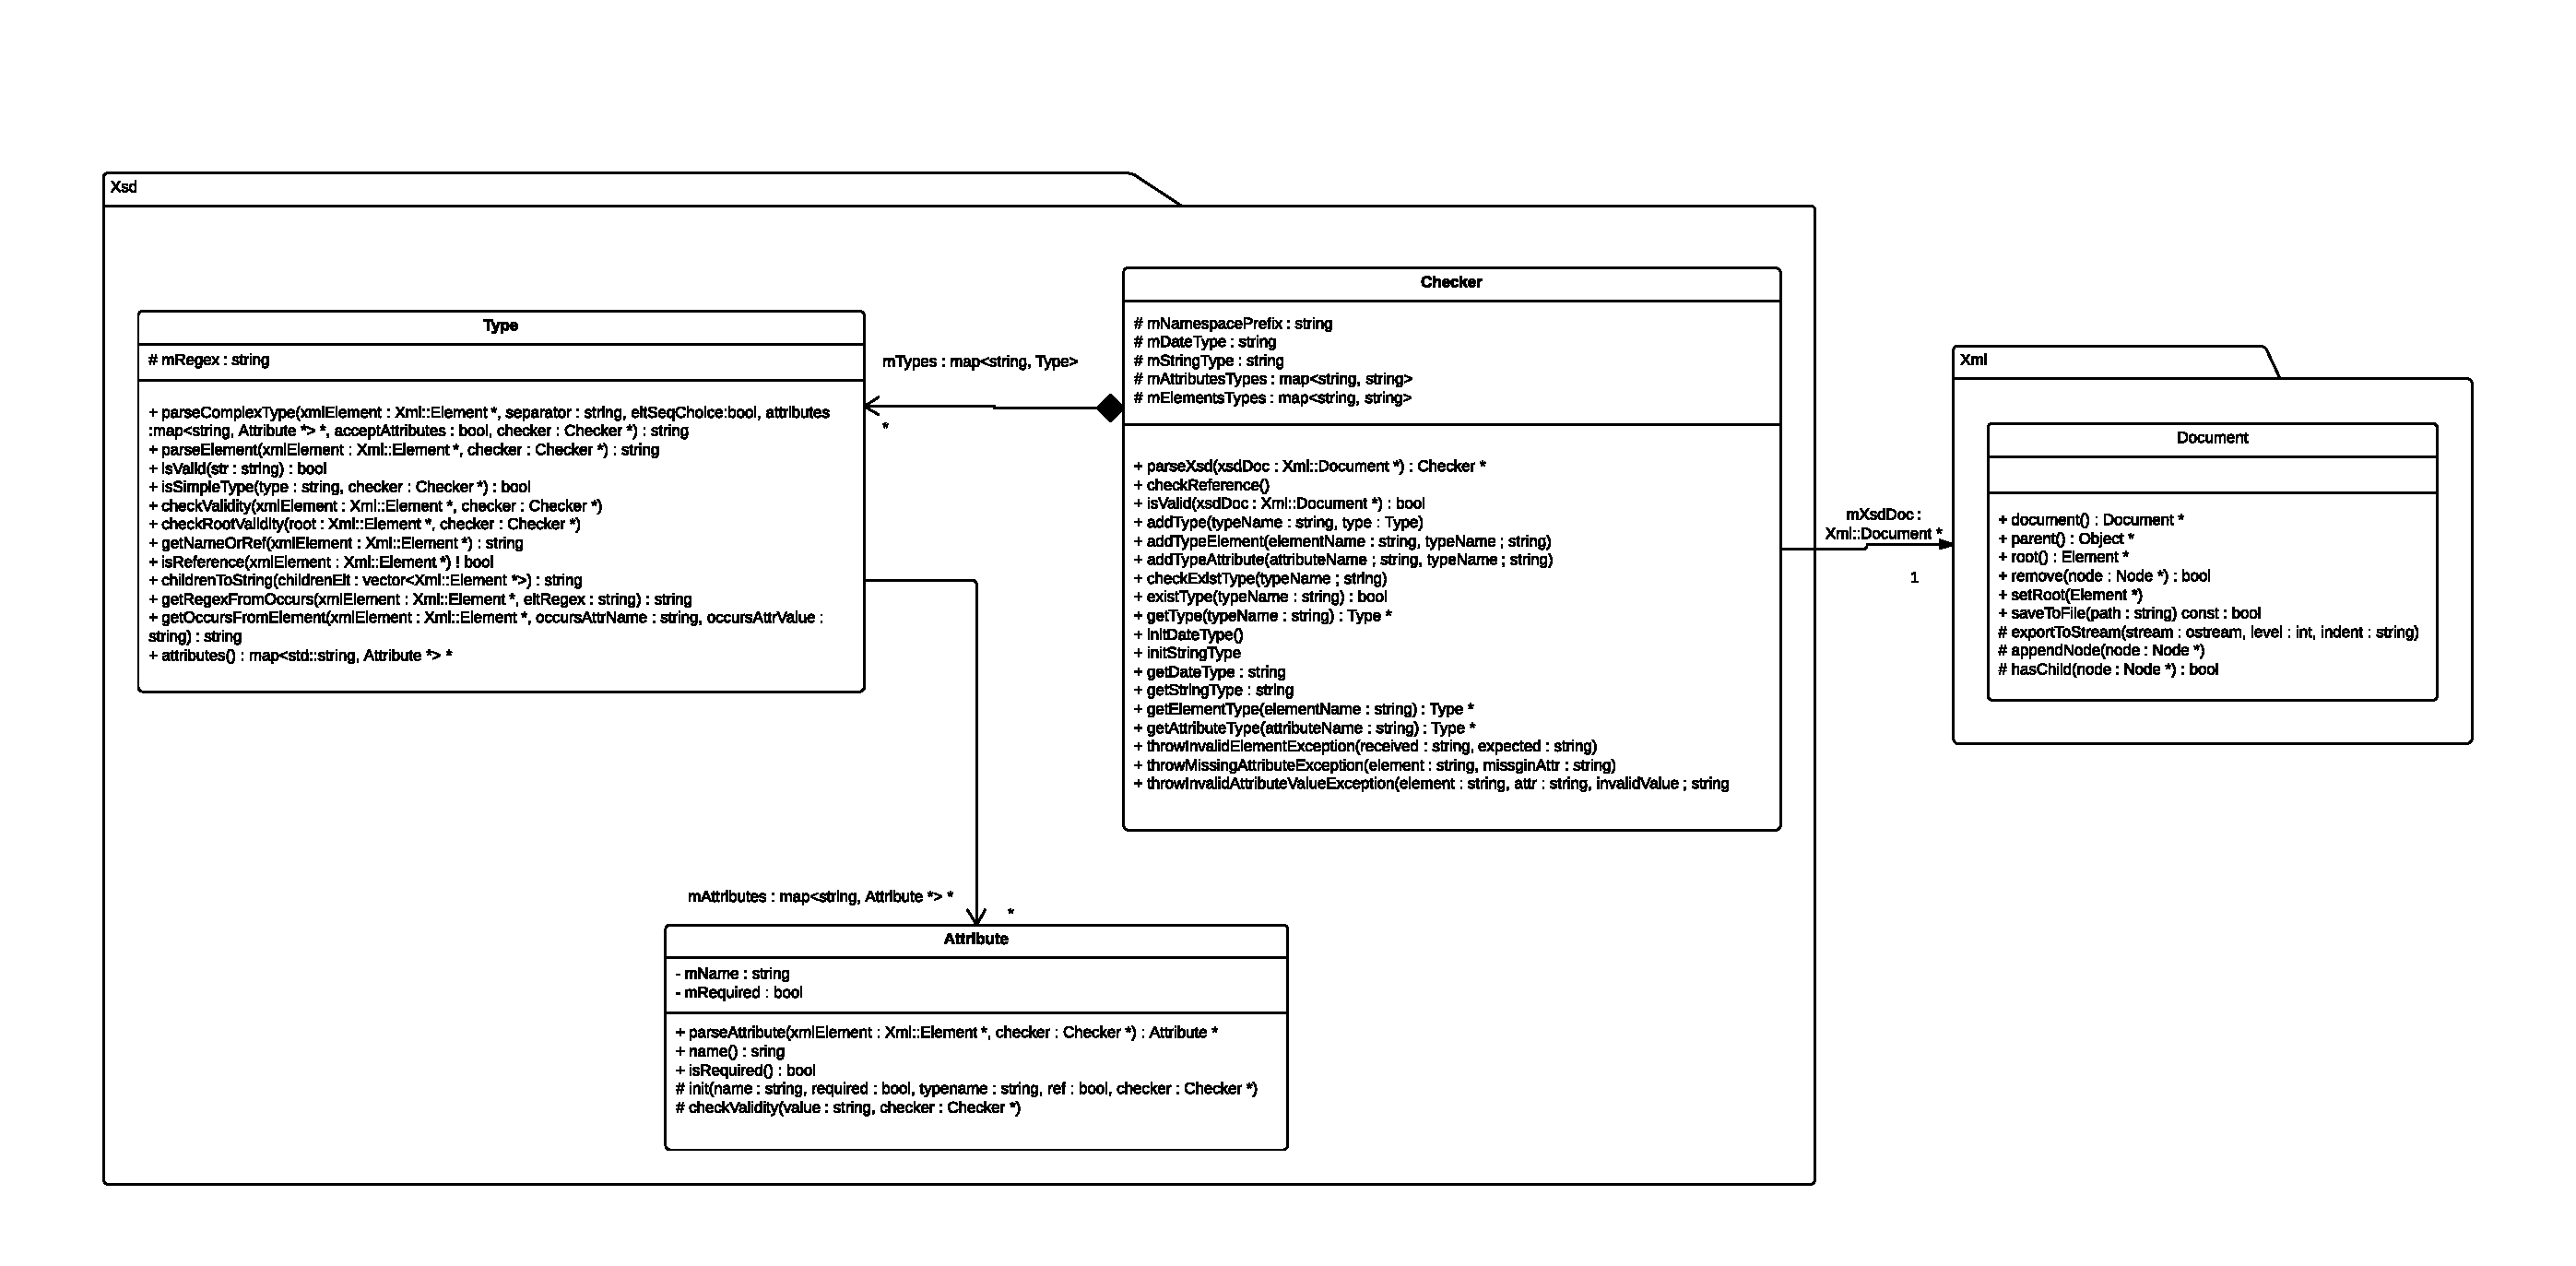
\includegraphics[width=1.1\linewidth]{images/xsd-uml.pdf}
        \caption{Diagramme de classe de la validation xsd}
        \label{classDiagram}
    \end{figure}

    \subsection{Classes}

        \subsubsection{Checker}

        \subsubsection{Type}

        \subsubsection{Attribute}

\section{Algorithme}

